\chapter{Конструкторский раздел}

В данном разделе приведено описание сущностей и диаграмма проектируемой базы данных, описание проектируемых ограничений целостности базы данных, описание проектируемых триггеров и описание проектируемой ролевой модели.

\section{Описание сущностей базы данных}

Анализируя таблицу \ref{tab:er} и диаграмму сущностей базы данных (рисунок \ref{img:er}) формализуем сущности проектируемой базы данных. В таблицах \ref{tab:tractor} - \ref{tab:report} приведена формализация полей выделенных сущностей, указаны их типы и ограничения.



На рисунке \ref{img:erdb} приведена ER-диаграмма проектируемой базы данных.


\begin{table}[H]
    \centering
  
    \begin{tabular}{|c|c|c|c|} \hline 
         \textbf{поле}&  \textbf{тип}&  \textbf{ограничения}& \textbf{описание}\\ \hline 
         id &  \makecell{уникальный \\ идентификатор} & \makecell{not null,\\ primary key} & \makecell{идентификатор \\ трактора}\\ \hline 
         model&  строка&  not null& название модели\\ \hline 
         releaseyear& дата&  not null& \makecell{год создания\\ модели}\\ \hline 
         enginetype&  строка&  not null& тип двигателя\\ \hline 
         enginemodel&  строка&  not null& модель двигателя\\ \hline 
         enginepower&  целое число&  not null& \makecell{мощность двигателя\\ в лошадиных силах}\\ \hline 
         fronttiresize&  целое число&  not null& \makecell{диаметр передних\\ колес в дюймах}\\ \hline 
         backtiresize&  целое число&  not null& \makecell{диаметр задних\\ колес в дюймах}\\ \hline 
         wheelsamount&  целое число&  not null& количество колес\\ \hline
 tankcapacity& целое число& not null&\makecell{вместимость\\ бензобака\\ в литрах}\\\hline
 ecologicalstandart& строка& not null& \makecell{эклолгический\\ стандарт}\\\hline
 length& \makecell{вещественное \\число}& not null&длина в метрах\\ \hline 
 width& \makecell{вещественное \\число}& not null&ширина в метрах\\\hline
 cabinheight& \makecell{вещественное \\число}& not null&\makecell{высота по кабине\\ в метрах}\\\hline
    \end{tabular}
    \caption{Формализация полей таблицы тракторов}
    \label{tab:tractor}
\end{table}



\begin{table}[H]
    \centering
    \begin{tabular}{|c|c|c|c|} \hline 
        \textbf{поле}&  \textbf{тип}&  \textbf{ограничения}& \textbf{описание}\\ \hline 
         id&  \makecell{уникальный \\ идентификатор}&  \makecell{not null,\\ primary key}& \makecell{идентификатор\\ производственной\\ линии}\\ \hline 
         name&  строка&  not null& название линии\\ \hline 
         length&  целое число&  not null& длина в мм\\ \hline 
         width&  целое число&  not null& ширина в мм\\ \hline 
         height&  целое число&  not null& высота в мм\\ \hline 
         status&  строка&  not null& статус\\ \hline 
         production&  целое число&  not null& \makecell{количество\\ произведенных\\ тракторов в месяц}\\ \hline 
         downtime&  целое число&  not null& \makecell{время простоя\\ в минутах}\\ \hline 
         inspectionsamount&  целое число&  not null& \makecell{требуемое\\ количество \\техосмотров в год}\\ \hline 
         lastinspection&  дата&  not null& \makecell{дата последнего\\ техосмотра}\\ \hline
 nextinspection& дата& not null&\makecell{дата следующего \\техосмотра}\\\hline
 defectrate& целое число& not null&\makecell{процент брака}\\\hline
    \end{tabular}
    \caption{Формализация полей таблицы производственных линий}
    \label{tab:assemblyline}
\end{table}



\begin{table}[H]
    \centering
    \begin{tabular}{|c|c|c|c|} \hline 
        \textbf{поле}&  \textbf{тип}&  \textbf{ограничения}& \textbf{описание}\\ \hline 
         id&  \makecell{уникальный \\ идентификатор}&  \makecell{not null, primary key}& \makecell{идентификатор \\пользователя}\\ \hline 
         name&  строка&  not null& имя\\ \hline 
         surname&  строка&  not null& фамилия\\ \hline 
         fathername&  строка&  not null& отчество\\ \hline 
         department&  строка&  not null& отдел\\ \hline 
         email&  строка&  not null& почта\\ \hline 
         password&  \makecell{хэшированная стрка}&  not null& пароль\\ \hline 
         dateofbirth&  дата&  not null& дата рождения\\ \hline 
         sex&  строка &  not null& пол \\ \hline 
         role&  строка&  not null& должность\\ \hline
    \end{tabular}
    \caption{Формализация полей таблицы сотрудников}
    \label{tab:user}
\end{table}



\begin{table}[H]
    \centering
    \begin{tabular}{|c|c|c|c|} \hline 
         \textbf{поле}&  \textbf{тип}&  \textbf{ограничения}& \textbf{описание}\\ \hline 
         id&  \makecell{уникальный \\ идентификатор}&  \makecell{not null, primary key}& \makecell{идентификатор детали}\\ \hline 
         name&  строка&  not null& название\\ \hline 
         country&  строка&  not null& страна производитель\\ \hline 
          amount&  целое число&  not null& \makecell{количество на складе}\\ \hline 
         price&  \makecell{вещественное \\число}&  not null& цена в рублях\\ \hline 
         length&  целое число&  not null& длина в мм\\ \hline 
         width&  целое число&  not null& ширина в мм\\ \hline 
         height&  целое число&  not null& высота в мм\\ \hline
    \end{tabular}
    \caption{Формализация полей таблицы деталей}
    \label{tab:detail}
\end{table}


\begin{table}[H]
    \centering
    \begin{tabular}{|c|c|c|c|} \hline 
        \textbf{поле}&  \textbf{тип}&  \textbf{ограничения}& \textbf{описание}\\ \hline 
         id&  \makecell{уникальный \\ идентификатор}&  \makecell{not null, primary key}& \makecell{идентификатор \\заказа деталей}\\ \hline 
         userid&  \makecell{уникальный \\ идентификатор}&  \makecell{not null, foreign key}& \makecell{идентификатор \\заказчика}\\ \hline 
         requestid&  \makecell{уникальный \\ идентификатор}&  \makecell{not null, foreign key}& \makecell{идентификатор\\ заявки для которой \\заказывают \\детали}\\ \hline 
         status& строка&  not null& \makecell{статус \\заказа}\\ \hline 
         totalprice&  \makecell{вещественное \\число}&  not null& цена\\ \hline 
         orderdate&  дата&  not null& дата заказа\\\hline
    \end{tabular}
    \caption{Формализация полей таблицы заказа деталей}
    \label{tab:orderdetail}
\end{table}


\begin{table}[H]
    \centering
    \begin{tabular}{|c|c|c|c|} \hline 
        \textbf{поле}&  \textbf{тип}&  \textbf{ограничения}& \textbf{описание}\\ \hline 
         id&  \makecell{уникальный \\ идентификатор}&  \makecell{not null,\\ primary key}& \makecell{идентификатор заявки \\на обслуживание}\\ \hline 
         lineid&  \makecell{уникальный \\ идентификатор}&  \makecell{not null,\\ foreign key}& \makecell{идентификатор \\производственной\\ линии}\\ \hline 
         userid&  \makecell{уникальный \\ идентификатор}&  \makecell{not null,\\ foreign key}& \makecell{идентификатор\\ сотрудника}\\ \hline 
         requestdate&  дата&  not null& дата заказа\\ \hline 
         status&  строка&  not null& статус \\ \hline 
         type&  строка&  not null& \makecell{статус}\\ \hline 
         description&  текст&  not null& описание заявки\\ \hline
    \end{tabular}
    \caption{Формализация полей таблицы заявки на обслуживание}
    \label{tab:request}
\end{table}


\begin{table}[H]
    \centering
    \begin{tabular}{|c|c|c|c|} \hline 
        \textbf{поле}&  \textbf{тип}&  \textbf{ограничения}& \textbf{описание}\\ \hline 
         id&  \makecell{уникальный \\ идентификатор}&  \makecell{not null,\\ primary key}& \makecell{идентификатор \\отчета об \\обслуживании}\\ \hline 
         lineid&  \makecell{уникальный \\ идентификатор}&  \makecell{not null,\\ foreign key}& \makecell{идентификатор \\производственной линии}\\ \hline 
         userid&  \makecell{уникальный \\ идентификатор}&  \makecell{not null,\\ foreign key}& \makecell{идентификатор сотрудника}\\ \hline 
         requestid&  \makecell{уникальный \\ идентификатор}&  \makecell{not null,\\ foreign key}& \makecell{идентификатор заявки}\\ \hline 
         opendate&  дата и время&  not null& \makecell{дата начала \\обслуживания}\\ \hline 
         closedate&  дата и время&  not null& \makecell{дата завеншения \\обслуживания}\\ \hline 
         totalprice&  \makecell{вещественное \\число}&  not null& цена ремонта\\ \hline 
         description&  текст&  not null& описание\\ \hline
    \end{tabular}
    \caption{Формализация полей таблицы отчета об обслуживании}
    \label{tab:report}
\end{table}

\begin{figure}[H]
    \centering
    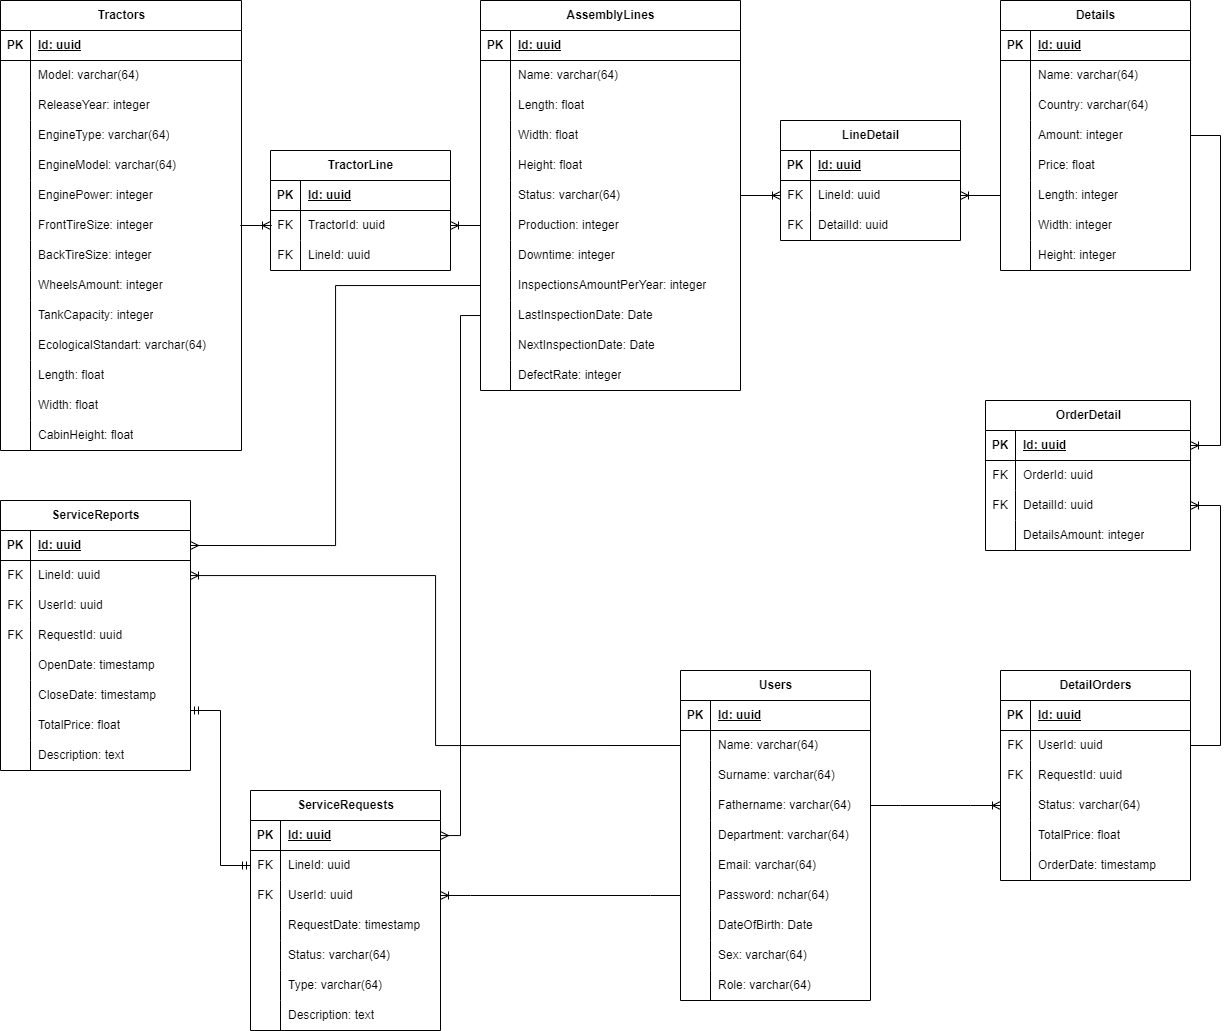
\includegraphics[width=1\textwidth]{inc/img/er.png}
    \caption{ER-диаграмма проектируемой базы данных}
    \label{img:erdb}
\end{figure}

\section{Описание проектируемых триггеров}

В проектируемой базе данных необходимо реализовать триггеры обновляющие значения некоторых полей после добавления новых записей в таблицы. 

На рисунке \ref{img:trigger2} приведен алгоритм триггера, обновляющего статус заявки на обслуживание после добавления записи в таблицу отчетов об обслуживании. Таким образом после публикации отчета об обслуживании статус проработанной заявки автоматически изменится на <<завершена>>.

На рисунке \ref{img:trigger3} приведен алгоритм триггера, обновляющего даты последнего и следующего техобслуживания, время простоя и статус производственной линии. При публикации отчета об обслуживании, будет вычислено количество часов прошедших с момента остановки работы производственной линии и это значение будет добавлено к полю DownTime, статус линии при этом будет изменен на <<работает>>. Если заявка на обслуживание, на основе которой был составлен отчет, имела тип <<техосмотр>>, то публикация отчета будет означать, что техосмотр был проведен, а значит необходимо занести информацию об этом в таблицу производственной линии. Так, после завершения техосмотра, его дата будет записана в поле LastInspectionDate и на основе данных о требуемой частоте техосмотров линии будет рассчитана дата следующего техосмотра.

На рисунке \ref{img:trigger4} приведен алгоритм триггера, обновляющего статус производственной линии при создании заявки на ее обслуживание. После публикации заявки на обслуживание статус производственной линии автоматически изменится на <<на обслуживании>>.


\begin{figure}[H]
    \centering
    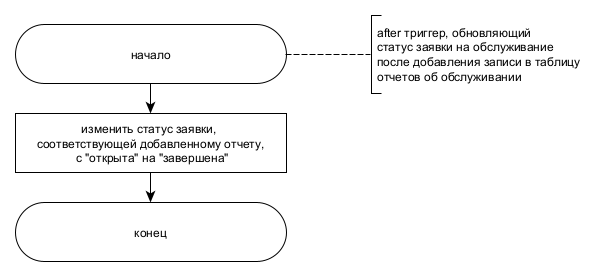
\includegraphics[width=0.85\textwidth]{inc/img/trigger2.png}
    \caption{Алгоритм триггера, обновляющего статус заявки на обслуживание}
    \label{img:trigger2}
\end{figure}

\begin{figure}[H]
    \centering
    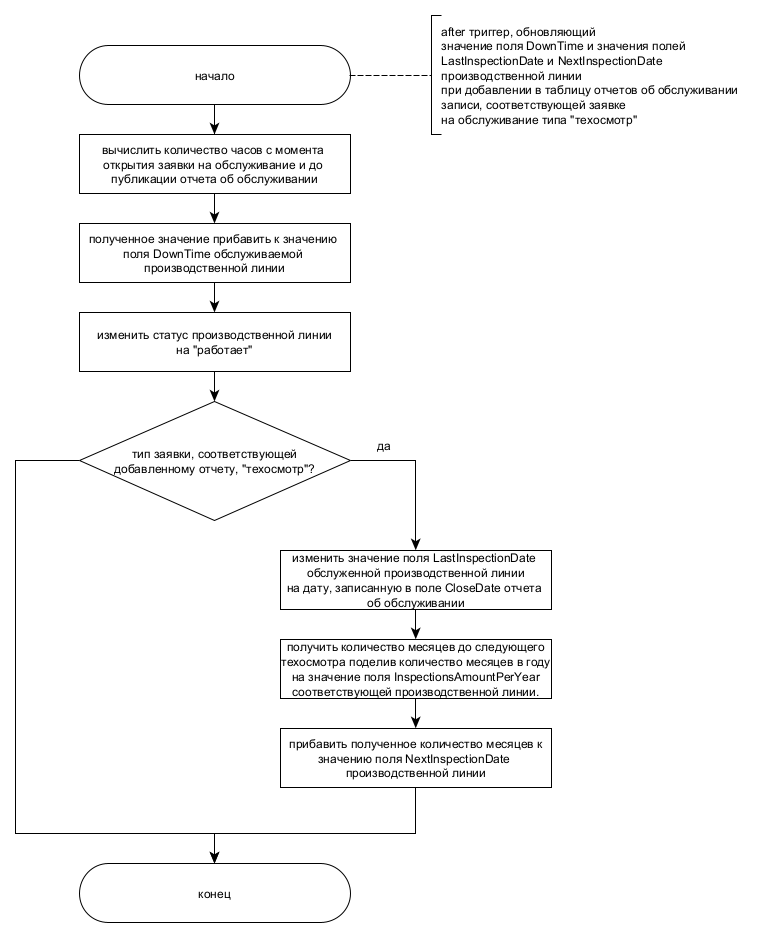
\includegraphics[width=1\textwidth]{inc/img/trigger3.png}
    \caption{Алгоритм триггера, обновляющего даты последнего и следующего техобслуживания, времени простоя и статуса производственной линии}
    \label{img:trigger3}
\end{figure}

\begin{figure}[H]
    \centering
    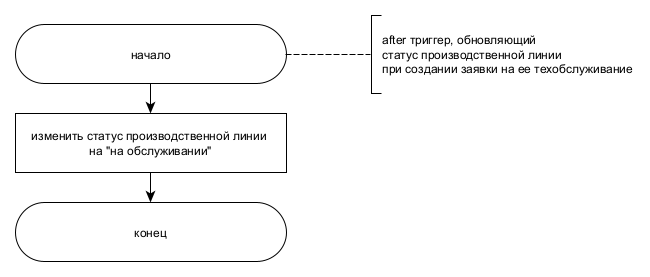
\includegraphics[width=0.85\textwidth]{inc/img/trigger4.png}
    \caption{Алгоритм триггера, обновляющего статус производственной линии}
    \label{img:trigger4}
\end{figure}

\section{Описание проектируемой ролевой модели}

Для эффективного и безопасного взаимодействия пользователей с базой данных была разработана ролевая модель, определяющая функционал доступный каждому типу пользователей.

В таблице \ref{tab:rolemodel} описан уровень доступа для каждого типа пользователя. Символом <<(*)>> обозначим все таблицы базы данных. Таким образом у администратора есть полный доступ ко всем таблицам. Символом <<\textbf{---}>> обозначим отсутствие таблиц для данного типа доступа.




\begin{table}[H]
    \centering
    \begin{tabular}{|c|c|c|c|} \hline  
         &  \textbf{SELECT}& \textbf{UPDATE} & \textbf{INSERT} \\ \hline  
         \textbf{\makecell{Оператор\\ производства}}&  \makecell{Tractors,\\ AssemblyLines,\\ ServiceReports,\\ ServiceRequests}& \makecell{AssemblyLines,\\ ServiceReqests, \\ Users} & \makecell{ServiceRequests}\\ \hline  
         \textbf{\makecell{Специалист\\ по обслуживанию}}& \makecell{Tractors,\\ AssemblyLines,\\ ServiceRequests,\\ ServiceReports,\\ Details,\\ DetailOrders} & \makecell{DetailOrders,\\ ServiceReports,\\ Users} & \makecell{ServiceReports, \\DetailOrders} \\ \hline  
         \textbf{Администратор}& (*) & (*) & (*)\\ \hline  
        \textbf{\makecell{Неавторизованный\\ пользователь}} & \textbf{---} & \textbf{---} & Users \\ \hline 
    \end{tabular}
    \caption{Описание проектируемой ролевой модели}
    \label{tab:rolemodel}
\end{table}

\subsection*{Вывод}

В данном разделе была проведена формализация сущностей и построена диаграмма проектируемой базы данных, спроектирована ролевая модель и триггеры.

